\section{内网资源}

\subsection{校园网}

BUPT的校园网也许不是最好的,但一定是最便宜的(指完全免费)。

北邮的几个校区共用一个超过40Gbps的聚合出口带宽,一般来说你的设备的网速都可以跑满无线或者有线连接本身的带宽,据称,即使在最高峰的时候,出口带宽也从未用满过(不过不要指望这会使你抢课的时候拥有什么优势)。

基本上沙河校区的建筑内都有WiFi的覆盖,室外也在逐步增加覆盖。在校园内覆盖了无线网络的区域,一般可以搜索到BUPT-mobile、BUPT-portal和BUPT-guest三个网络\footnote{在S1-S3楼内则是BUPT-SH-mobile和BUPT-SH-portal这两个WiFi 6标准的网络,连接速度更快}。一般手机平板等移动设备连接mobile,PC端连接portal(其实随便连都行),而guest不使用。初次使用需要在校园网服务网站上用学号登录,具体的初始密码会另行通知大家。

在校外必须使用学校的VPN才能访问内网的资源。可以使用\href{https://webvpn.bupt.edu.cn/}{WebVPN},也可以使用专门的客户端。目前客户端VPN正在计划更换,估计在开学前后就能用上了。

\subsection{常用网站}

\subsubsection*{可以直接访问的网站}
\begin{itemize}
    \item \href{https://www.bupt.edu.cn/}{北邮官网}:北京邮电大学的官方网站。
    \item \href{https://webvpn.bupt.edu.cn/}{WebVPN系统}:使用浏览器访问内网资源,无需安装客户端和插件,支持电脑和手机直接使用。
    \item \href{https://ucloud.bupt.edu.cn/}{云邮教学空间}:新开通的一个教学平台,部分课程会在里面发放资料、提交作业甚至考试。根据反馈,这个平台还有很多bug,不少同学被坑。
\end{itemize}

\subsubsection*{需要通过VPN或在校园网环境下访问的内网资源}
\begin{itemize}
    \item \href{http://my.bupt.edu.cn/}{信息门户}:发布校内通知、新闻等,也整合了各个网站系统的入口。勤看信息门户有助于不错过重要通知。
    \item \href{http://10.3.8.216/index}{校园网认证网关}:通过BUPT-portal上网需要登录,一般会自动跳转到此。
    \item \href{https://jwgl.bupt.edu.cn/}{本科生教务系统}:查课表考表成绩学分、抢课退补选等等,都在教务系统。
    \item \href{https://service.bupt.edu.cn/}{网上服务大厅}:线上办理各种手续的地方。\sout{甚至可以在线申请退学}
    \item \href{https://iclass.bupt.edu.cn/}{“爱课堂”教学平台}:部分科目的老师用来进行线上分发教学资料、收发作业和在线考试的平台。
\end{itemize}

\subsubsection*{其他相关的网络平台}
\begin{itemize}
    \item \href{https://mail.bupt.edu.cn/}{北邮邮箱}:开学后可以注册,适合用来做你自己学术专用的邮箱。带有@bupt.edu.cn后缀的邮箱被称为教育邮箱,可以用来申请很多对学生免费的资源。按教育部要求,教育邮箱会在毕业半年后被收回,转为@bupt.cn后缀的校友邮箱。
    \item \href{https://bbs.byr.cn/}{北邮人论坛}:最早的中文校园BBS之一,可以注册一个账号与其他同学交♂流,具体见下。
    \item \href{https://byr.pt/}{BYRBT}:知名的PT站,只有使用非国内三大运营商的IPv6地址才能访问,具体见下。
    \item \href{http://tv.byr.cn/show}{北邮人IPTV}:卫星电视直播站,可以看到很多台的电视直播,有的校园活动也会在上面转播,不过好像不太稳定(摊手
\end{itemize}

\subsubsection*{学校使用的一些公共网站平台}
\begin{itemize}
    \item \href{https://www.yuketang.cn/web}{雨课堂}:清华开发的平台,少部分的(现在几乎没有了)课程课件会发布在这里,可以使用微信登录。
    \item \href{https://www.ketangpai.com/}{课堂派}:部分老师收发作业用的平台,疫情期间的部分考试也使用此平台来发放、提交试卷。使用体验不算太好,有时会遇到卡顿。可以使用微信登录。
\end{itemize}
以上平台有微信小程序。
\begin{itemize}
    \item \href{https://passport.zhihuishu.com/}{智慧树}:网课平台之一,比较良心。
    \item \href{http://erya.mooc.chaoxing.com/}{超星尔雅}:网课平台之二,臭名昭著。\footnote{在2022年6月中旬发生了拖库事件,超星的数据库被全部泄露出去了,造成了很多人的隐私泄露}
    \item \href{https://www.icourse163.org/learn}{中国大学MOOC}:疫情期间才引入的网课平台,只有部分老师在里面开课。不过上面有很多其他大学的老师开放的在线课程,可以拓展一下知识面或作为课堂内容的补充。
\end{itemize}
以上平台有自己的App。


\faq{如何利用学校提供的学术资源?}

学校的图书馆系统中有“数据库导航”链接,由此可以进入查看学校所购买的学术资源数据库,包括(国内的)万方、知网和(国外的)IEL、Nature等。在校内(使用校园网的情况下),你可以直接进入这些网站并下载所需要的资料;在校外,你需要选择校外登录等方式,通过登录认证从而领用上述资源。以知网为例:

\begin{center}
    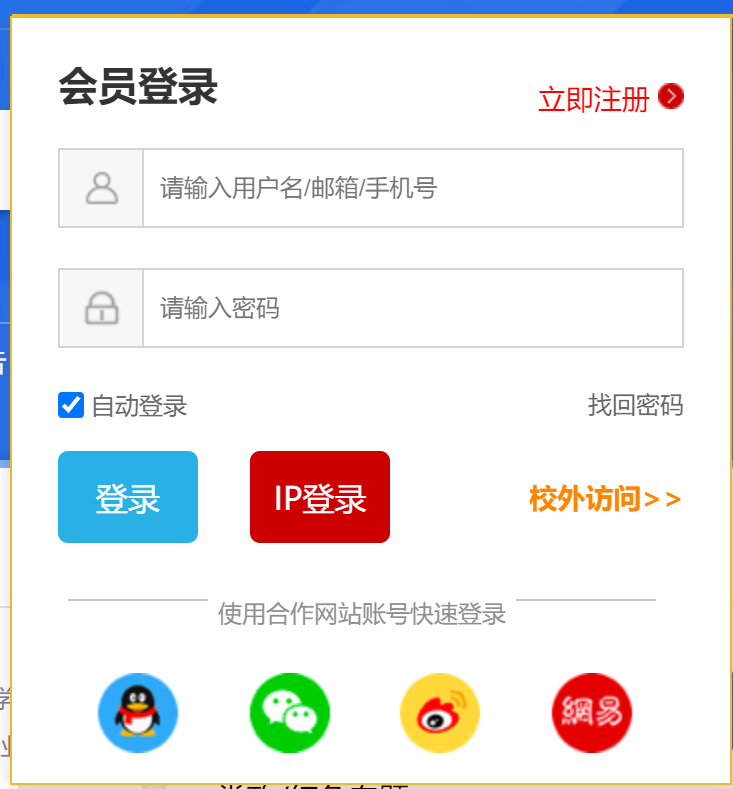
\includegraphics[width=0.4\textwidth]{images/cnki-login.png}
\end{center}

在校内,直接使用IP登录即可;在校外,需要点击校外访问,选择北京邮电大学,用校园网账号登录即可。在学校购买的数据库范围内下载论文、资料是全部免费的,学校每年给这些机构支付了天价的使用费,大家不需要自己花钱。

\faq{如何注册北邮人论坛?有什么用?}

使用你的北邮校园网帐号注册即可,一个学生号最多能注册三个账号,要经过手机验证后才能发帖。除了直接访问网站,也可以下载北邮人论坛的App,安卓、苹果都有,但体验不算太好。北邮人论坛是校内最重要的论坛,有学校老师入驻以确保言论合法且不具有攻击性。你可以在这里看到保研资讯、校内新闻、经验技术分享等等,是获取校内信息的重要途径。

\faq{BYRBT是什么?如何使用?}

BitTorrent是一种资源分享协议,它的宗旨是“我为人人,人人为我”。在BT资源站上,你可以下载到很多其他人分享的高质量资源(包括但不限于软件、电影、音乐、游戏、图书资料等——需要注意的是,这些资源并不一定都是正版),但同时你应当履行保存这些资源并利用你的网络上传给他人分享的义务。如果你只下载资源而不提供上传分享,或者随意在网站外分享得到的资源,BT站有权利封禁你的账号。

在符合要求的网络环境(例如校园网)下,就可以登录BYRBT。一个学号一般只能注册一个BT账号,所以一定要珍惜你的账号,不要因为滥用下载和随意外传资源而被封号。账号长时间不使用也会被删除(这个功能暂时没有开启),但是你可以手动“封存”它,在放假或者长时间不在学校前记得先封存账号,回到学校后解封它。

BYRBT是一个PT站,PT(Private Tracker)是一种基于私有BT Tracker服务器的资源传播形式,经授权的用户使用受允许的客户端进行种子制作与下载。要使用BYRPT提供的服务,就必须遵守站内的相关规则。注册并登录后你可以在网站上看到规则和常见问题,请仔细阅读。
